% KU Leuven latex presentation template
%
% © 2012 Michael Hofmann
%
% This work is licensed under the Creative Commons Attribution 3.0 Unported License.
% To view a copy of this license, visit
% http://creativecommons.org/licenses/by/3.0/ or send a letter to Creative
% Commons, 444 Castro Street, Suite 900, Mountain View, California, 94041, USA.

\documentclass[t,12pt,english
\ifx\beamermode\undefined\else,\beamermode\fi
]{beamer}
%\setbeameroption{show notes}
%\setbeameroption{show only notes}

\input{configuratie.tex}

\title{Ontwikkeling van een\\autonoom lijn-volgend\\racevoertuig}
\author{\mbox{De Bruycker Jorik} \and \mbox{Bolle Jonas}}
\date{09/05/18}
\institute{3ELICTE}

\begin{document}

\setbeamertemplate{background canvas}[title]

\begin{frame}[plain,noframenumbering]
    \titlepage
\end{frame}

\usedefaultcanvas

\emptyfooter

\begin{frame}{}
\begin{figure}[H]
	\centering
	\includegraphics[width=\textwidth,height=0.8\textheight,keepaspectratio]{robbie.png}
\end{figure}
\end{frame}

\begin{frame}[noframenumbering]{Inhoud}
        \tableofcontents
\end{frame}
\largefooter

%%%%%%%%%%%%%%%%%%%%%%%%%%%%%%%%%%%%%%%%%%%%%%%%%%%%%%%%%%%%%%%%%%%%%%%%%%%%%%%%%%
\section{Ontwerp custom Arduino-board}\label{sec:pcb}

\begin{frame}{Eigen Eagle-ontwerp}
\begin{figure}[H]
	\centering
	\includegraphics[width=\textwidth,height=0.8\textheight,keepaspectratio]{eigenschematic.png}
\end{figure}
\end{frame}

\begin{frame}{Eigen Eagle-ontwerp: Motor Shield}
\begin{figure}[H]
	\centering
	\includegraphics[width=\textwidth,height=0.8\textheight,keepaspectratio]{eigenschematicdeel1.png}
\end{figure}
\end{frame}

\begin{frame}{Eigen Eagle-ontwerp: Voeding}
\begin{figure}[H]
	\centering
	\includegraphics[width=\textwidth,height=0.8\textheight,keepaspectratio]{eigenschematicdeel2.png}
\end{figure}
\end{frame}

\begin{frame}{Eigen Eagle-ontwerp: Micro-Controller}
\begin{figure}[H]
	\centering
	\includegraphics[width=\textwidth,height=0.8\textheight,keepaspectratio]{eigenschematicdeel3.png}
\end{figure}
\end{frame}

\begin{frame}{Eigen Eagle-ontwerp van PCB}
\begin{figure}[H]
	\centering
	\begin{minipage}[b]{0.4\textwidth}
		\centering
		\includegraphics[width=\textwidth,height=0.8\textheight,keepaspectratio]{topboard.png}
	\end{minipage}
	\hfill
	\begin{minipage}[b]{0.4\textwidth}
		\centering
		\includegraphics[width=\textwidth,height=0.8\textheight,keepaspectratio]{bottomboard.png}
	\end{minipage}
\end{figure}
\end{frame}

\begin{frame}{Eigen PCB}
\begin{figure}[H]
	\centering
	\begin{minipage}[b]{0.4\textwidth}
		\centering
		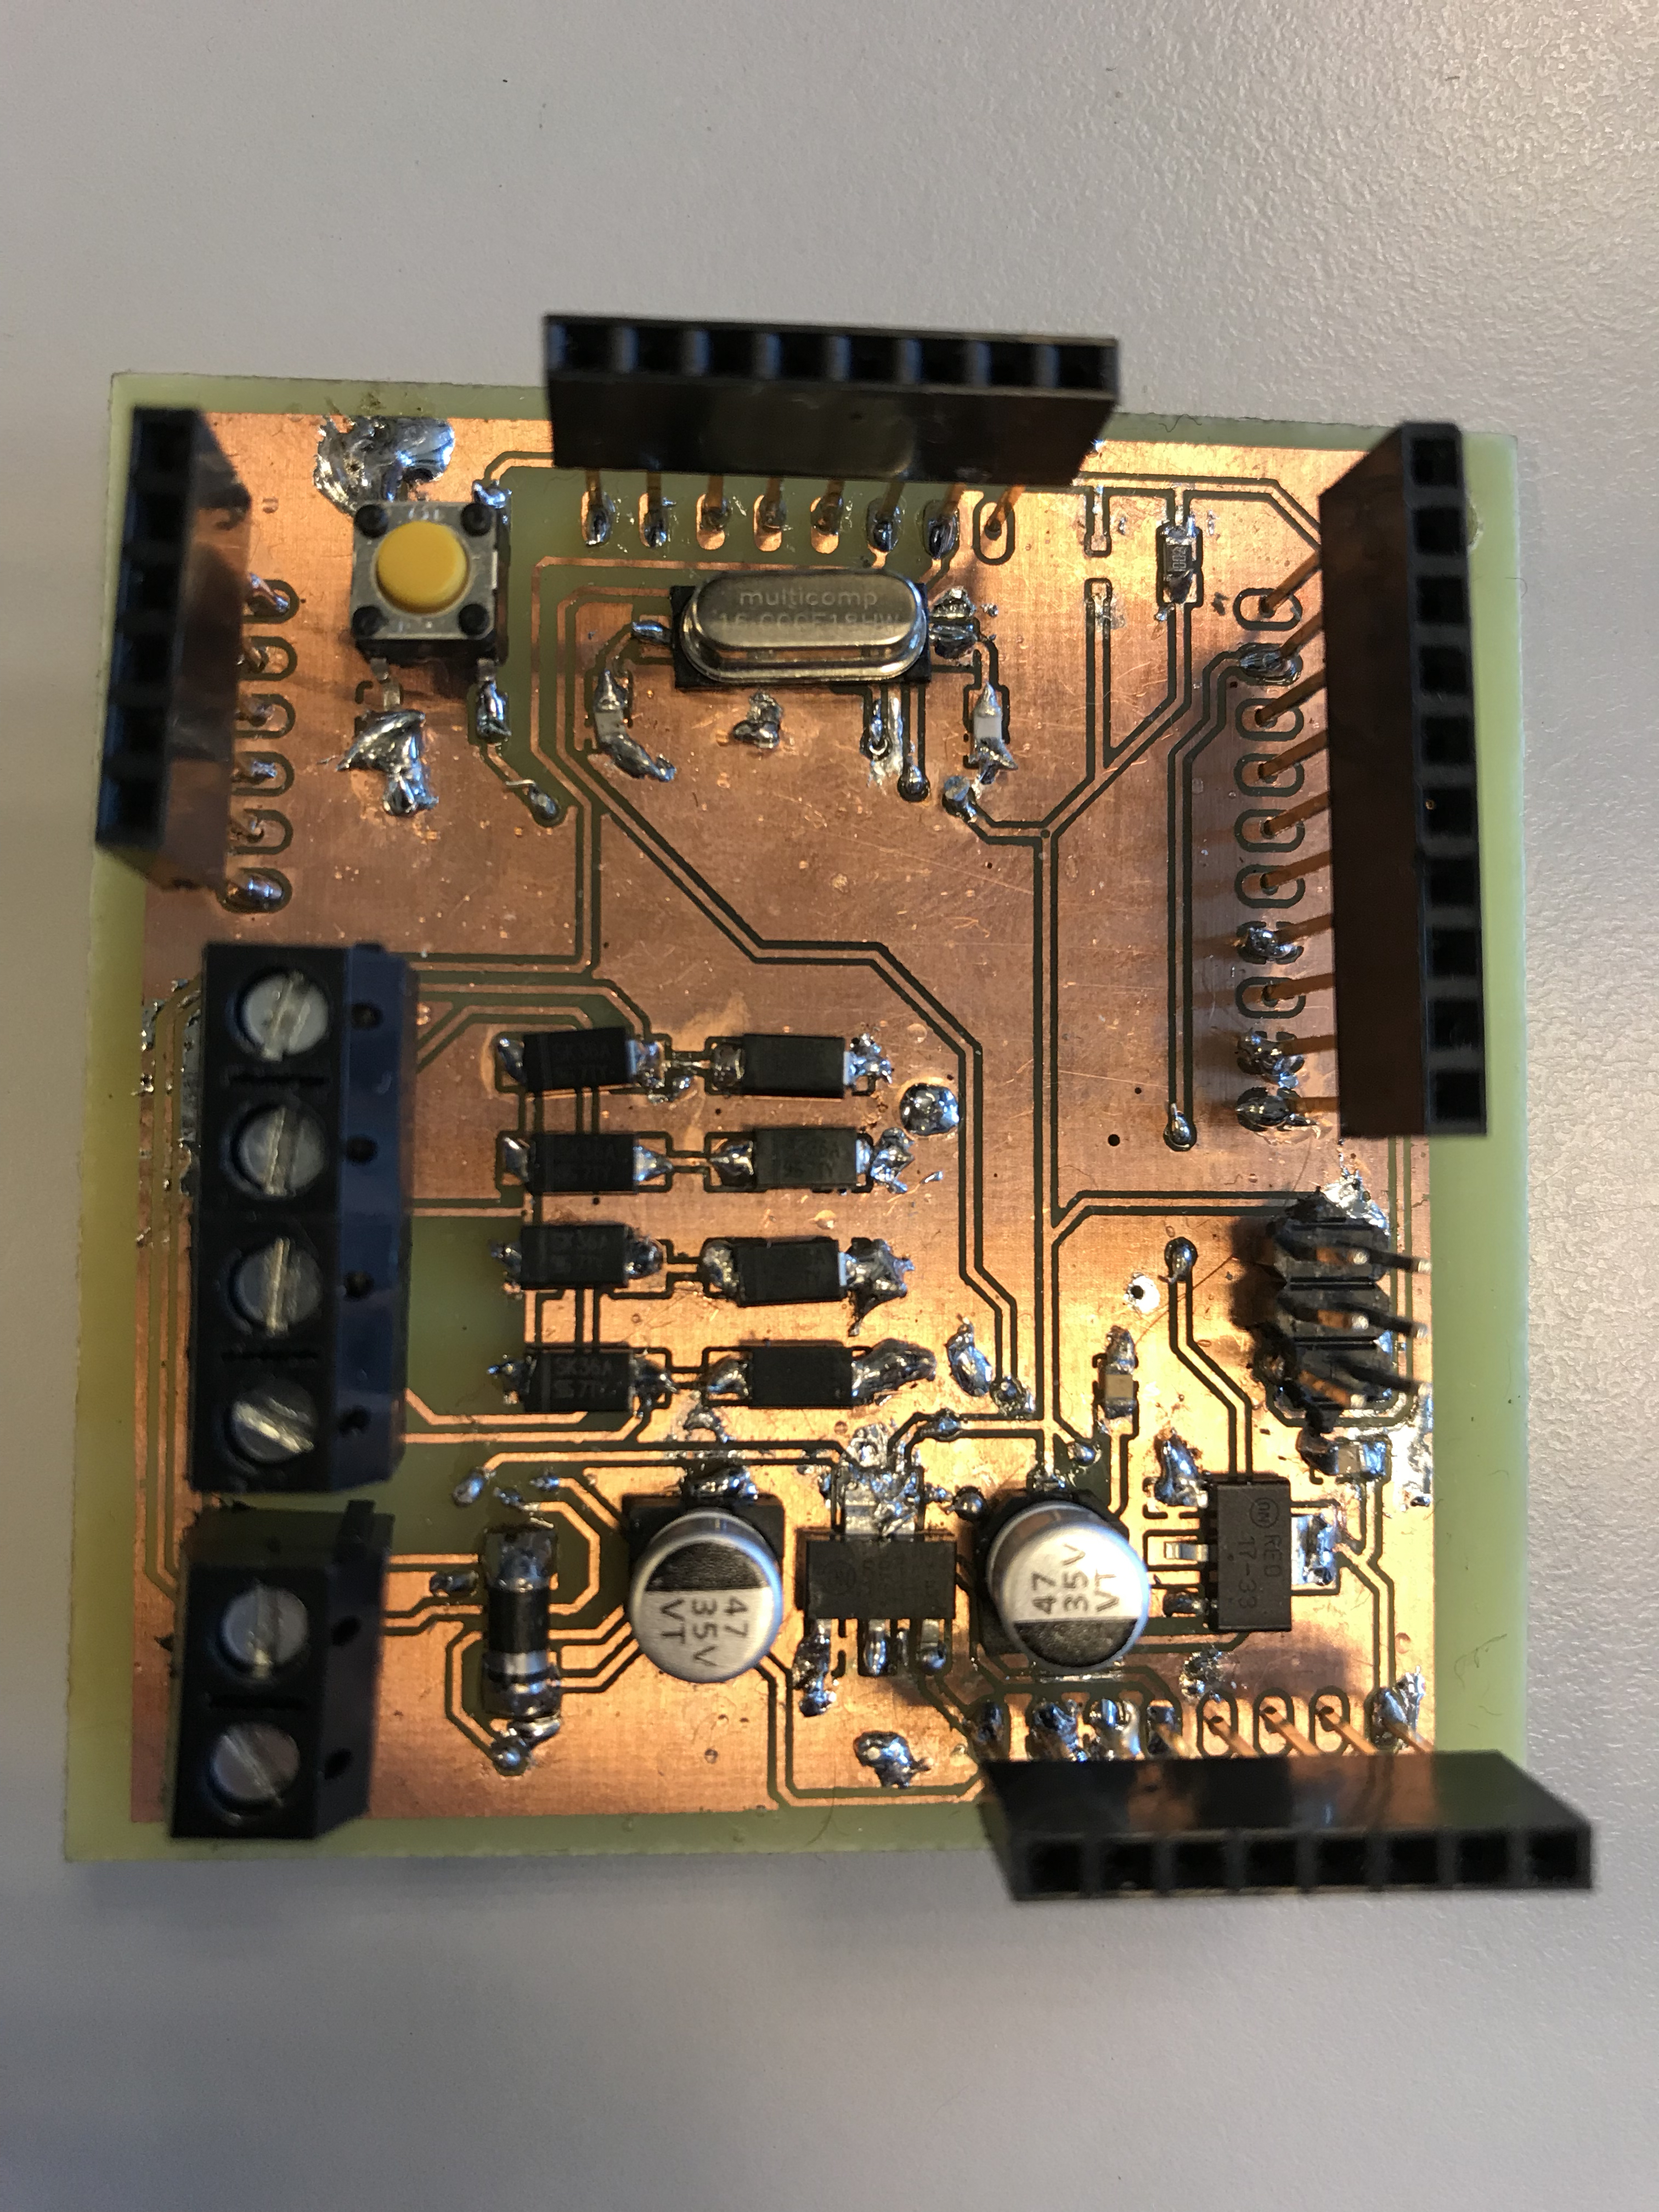
\includegraphics[width=\textwidth,height=0.8\textheight,keepaspectratio]{eigenpcbarduino.png}
	\end{minipage}
	\hfill
	\begin{minipage}[b]{0.4\textwidth}
		\centering
		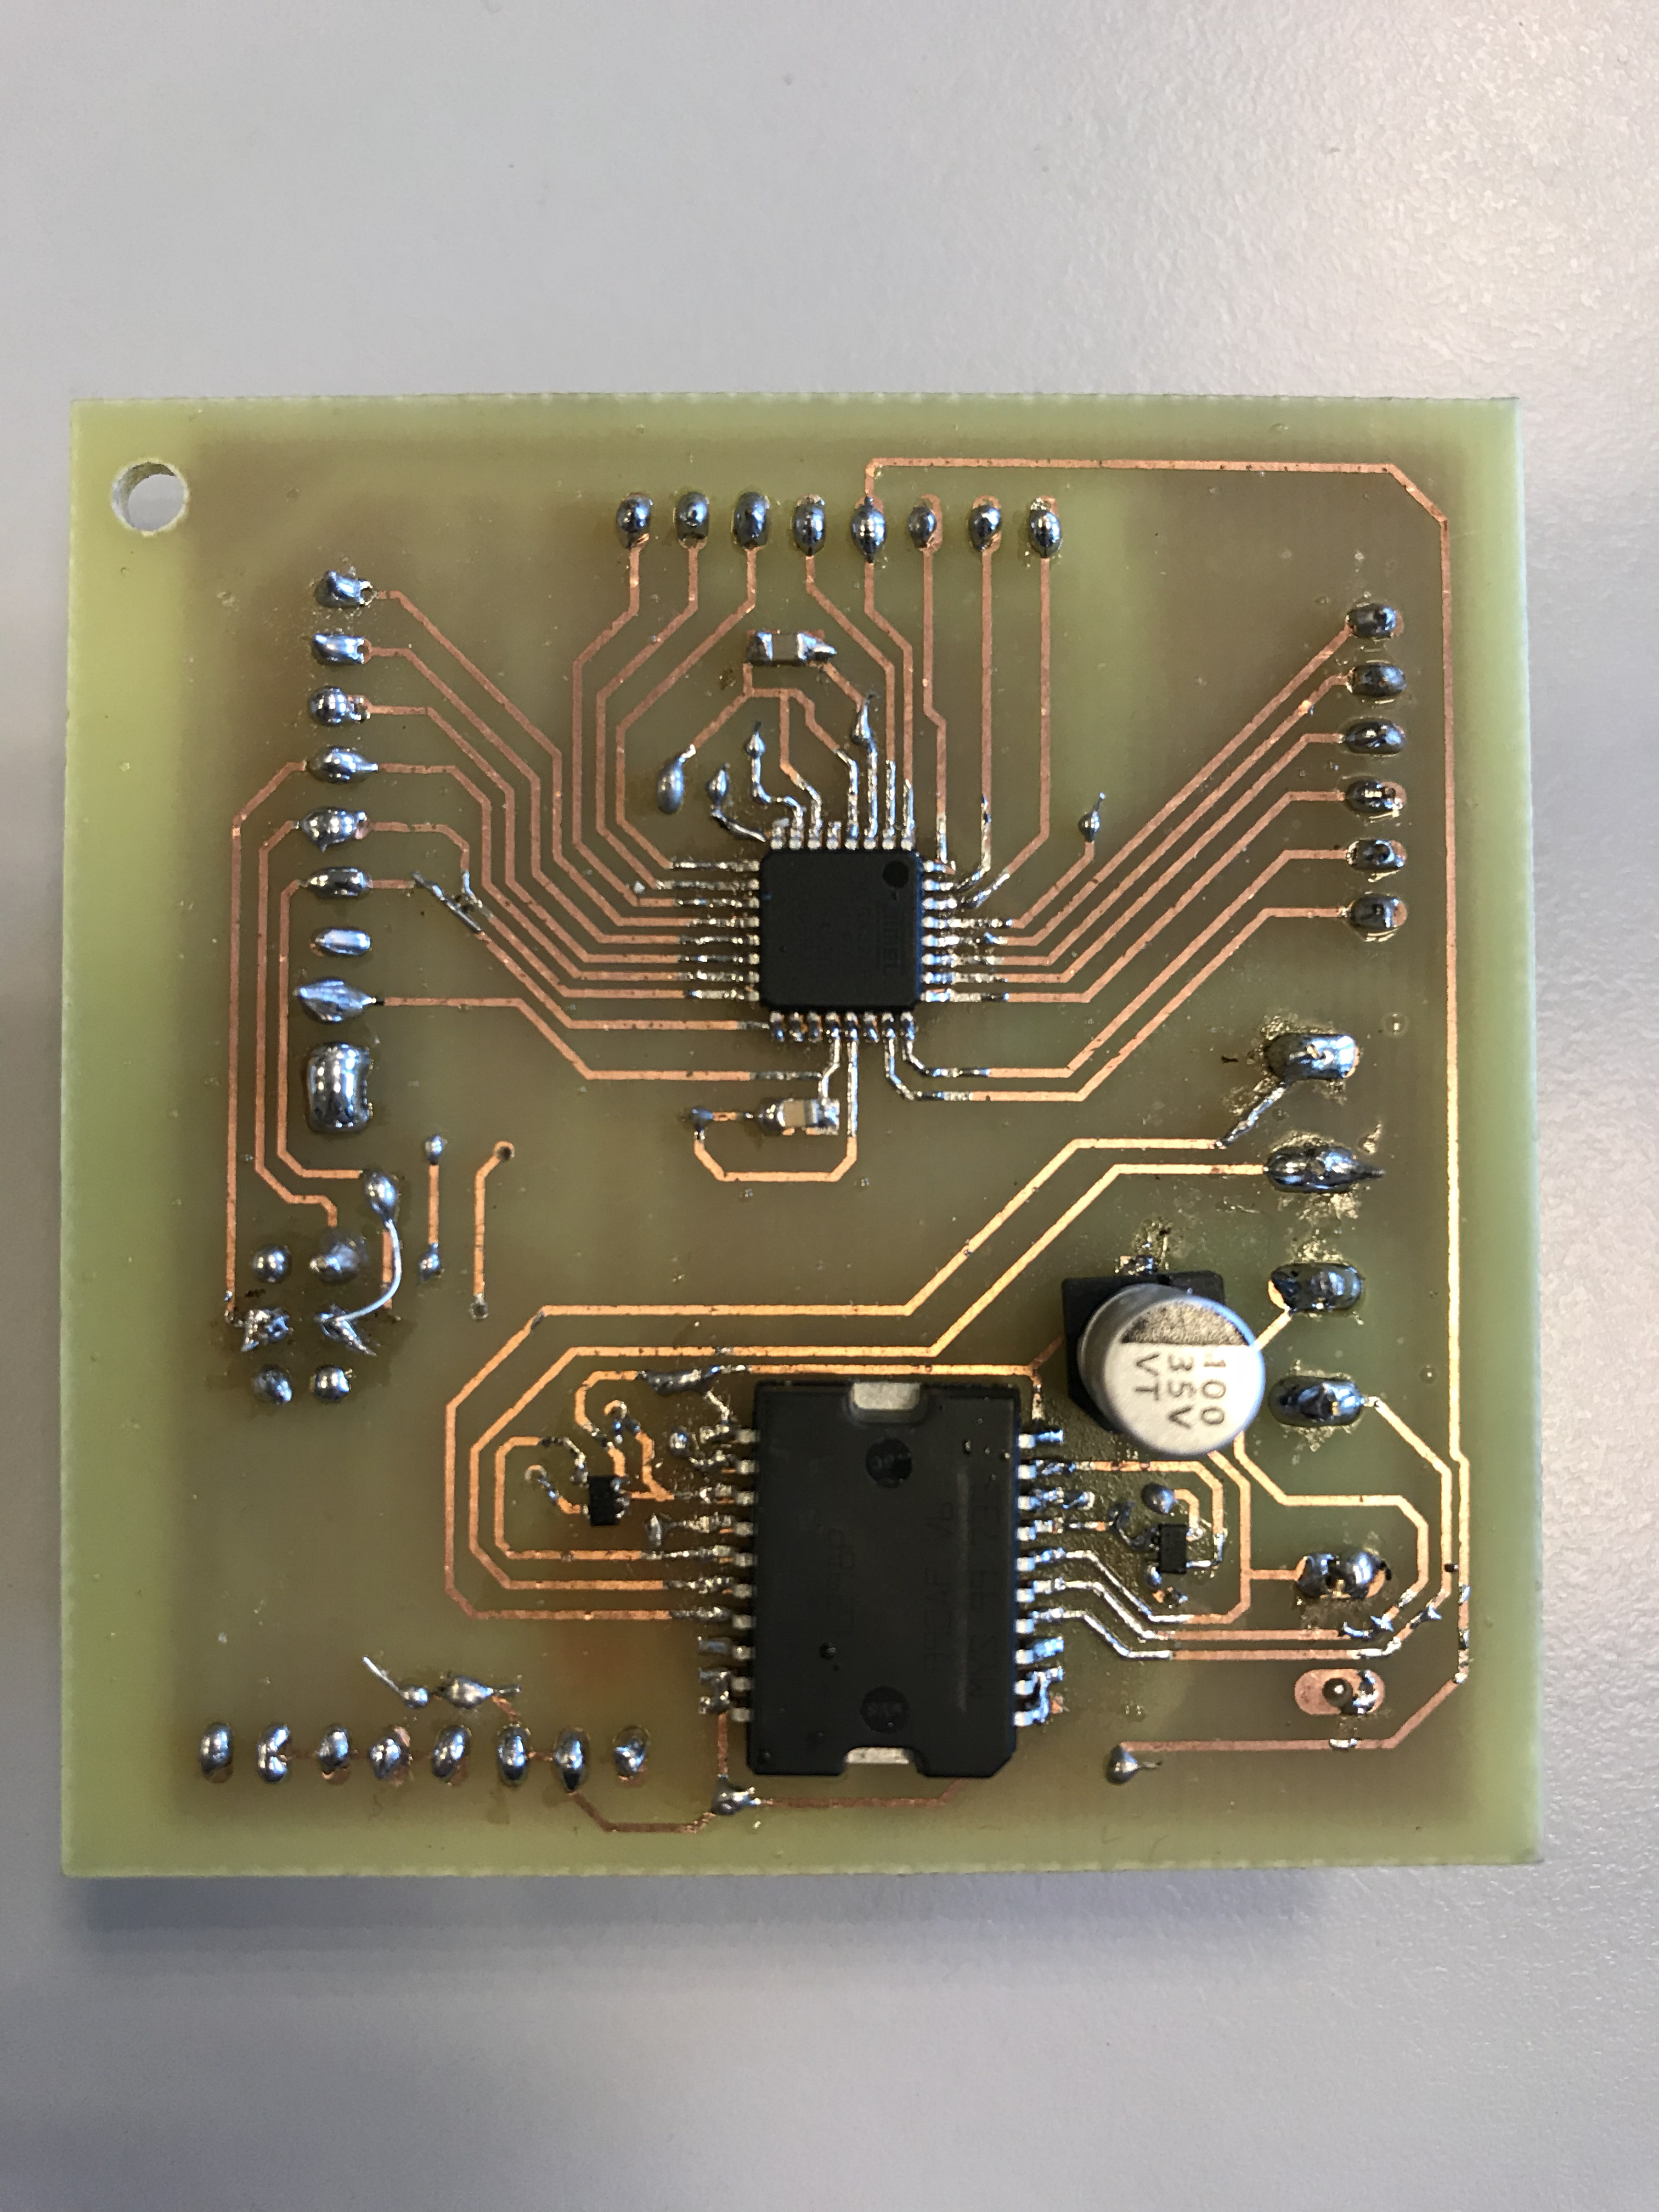
\includegraphics[width=\textwidth,height=0.8\textheight,keepaspectratio]{eigenpcb2.png}
	\end{minipage}
\end{figure}
\end{frame}

%%%%%%%%%%%%%%%%%%%%%%%%%%%%%%%%%%%%%%%%%%%%%%%%%%%%%%%%%%%%%%%%%%%%%%%%%%%%%%%%%%
\section{Infrarood-sensoren en sturen}
\begin{frame}{Sensor-cel}
\begin{figure}[H]
	\centering
	\includegraphics[width=\textwidth,height=0.8\textheight,keepaspectratio]{tcrt5000cel.png}
\end{figure}
\end{frame}

\begin{frame}{Inlezen aan de hand van Gray-code}
\begin{table}[H]
	\centering
	\renewcommand{\arraystretch}{1}
	\begin{tabular}{|l|l|l|l|l|l|}
		\hline
		\# & Select 2 & Select 1 & Select 0 & MUX-pin & Sensor      \\ \hline
		0  & 0            & 0            & 0            & 13      & Vooraan 2   \\ \hline
		1  & 0            & 0            & 1            & 14      & Vooraan 3   \\ \hline
		3  & 0            & 1            & 1            & 12      & Vooraan 1   \\ \hline
		2  & 0            & 1            & 0            & 15      & Vooraan 4   \\ \hline
		6  & 1            & 1            & 0            & 2       & Achteraan 3 \\ \hline
		7  & 1            & 1            & 1            & 7       & Achteraan 2 \\ \hline
		5  & 1            & 0            & 1            & 5       & Achteraan 1 \\ \hline
		4  & 1            & 0            & 0            & 7       & Achteraan 4 \\ \hline
	\end{tabular}
\end{table}
\end{frame}

\begin{frame}{Foutwaarde berekenen}
\begin{table}[H]
	\centering
	\begin{tabular}{lllll}
		\hline
		\multicolumn{1}{|l|}{}           & \multicolumn{1}{l|}{Vooraan 1}   & \multicolumn{1}{l|}{Vooraan 2}   & \multicolumn{1}{l|}{Vooraan 3}   & \multicolumn{1}{l|}{Vooraan 4}   \\ \hline
		\multicolumn{1}{|l|}{Gewicht} & \multicolumn{1}{l|}{-3}          & \multicolumn{1}{l|}{-1}          & \multicolumn{1}{l|}{1}           & \multicolumn{1}{l|}{3}           \\ \hline
		&                                  &                                  &                                  &                                  \\ \hline
		\multicolumn{1}{|l|}{}           & \multicolumn{1}{l|}{Achteraan 1} & \multicolumn{1}{l|}{Achteraan 2} & \multicolumn{1}{l|}{Achteraan 3} & \multicolumn{1}{l|}{Achteraan 4} \\ \hline
		\multicolumn{1}{|l|}{Gewicht} & \multicolumn{1}{l|}{3}           & \multicolumn{1}{l|}{1}           & \multicolumn{1}{l|}{-1}          & \multicolumn{1}{l|}{-3}           \\ \hline
	\end{tabular}
\end{table}

\begin{align*}
E_{fout} = \frac{\sum\limits_{i=1}^{4}S_{i}\cdot G_{i}}{\sum\limits_{i=1}^{4}S_{i}} &&
\begin{aligned}
S_i=\text{Sensorwaarde}\\
G_i=\text{Gewicht sensor}
\end{aligned}
\end{align*}
\end{frame}

\begin{frame}{PID-regeling}
\begin{gather*}
F = K_P \cdot E_P + K_I \cdot E_I + K_D \cdot E_D\\
\end{gather*}
\begin{itemize}
	\item[] $F$ = factor bijsturen motoren
	\item[] $E_P = E_{totaal}$ = proportionele term
	\item[] $E_I = \sum E_{totaal}$ = integrerende term
	\item[] $E_D = E_{totaal} - E_{totaal,vorig}$ = differenti\"erende term
	\item[] $K$ = constante waarden om invloed term te schalen 
\end{itemize}

\end{frame}

%%%%%%%%%%%%%%%%%%%%%%%%%%%%%%%%%%%%%%%%%%%%%%%%%%%%%%%%%%%%%%%%%%%%%%%%%%%%%%%%%%
\section{Hall-sensor en snelheidsmeting}
\begin{frame}{Snelheidsmeting met Hall-sensor}
\begin{columns}
	\begin{column}{0.5\textwidth}
		\begin{gather*}
		v=\frac{\Delta x}{\Delta t} = \frac{\frac{C}{2}\cdot\pi\cdot D}{\Delta t}
		\end{gather*}
		$\Delta x$ = afgelegde weg\\
		$\Delta t$ = tijdsinterval\\
		$C$ = aantal ompolingen sensor
		\centering
		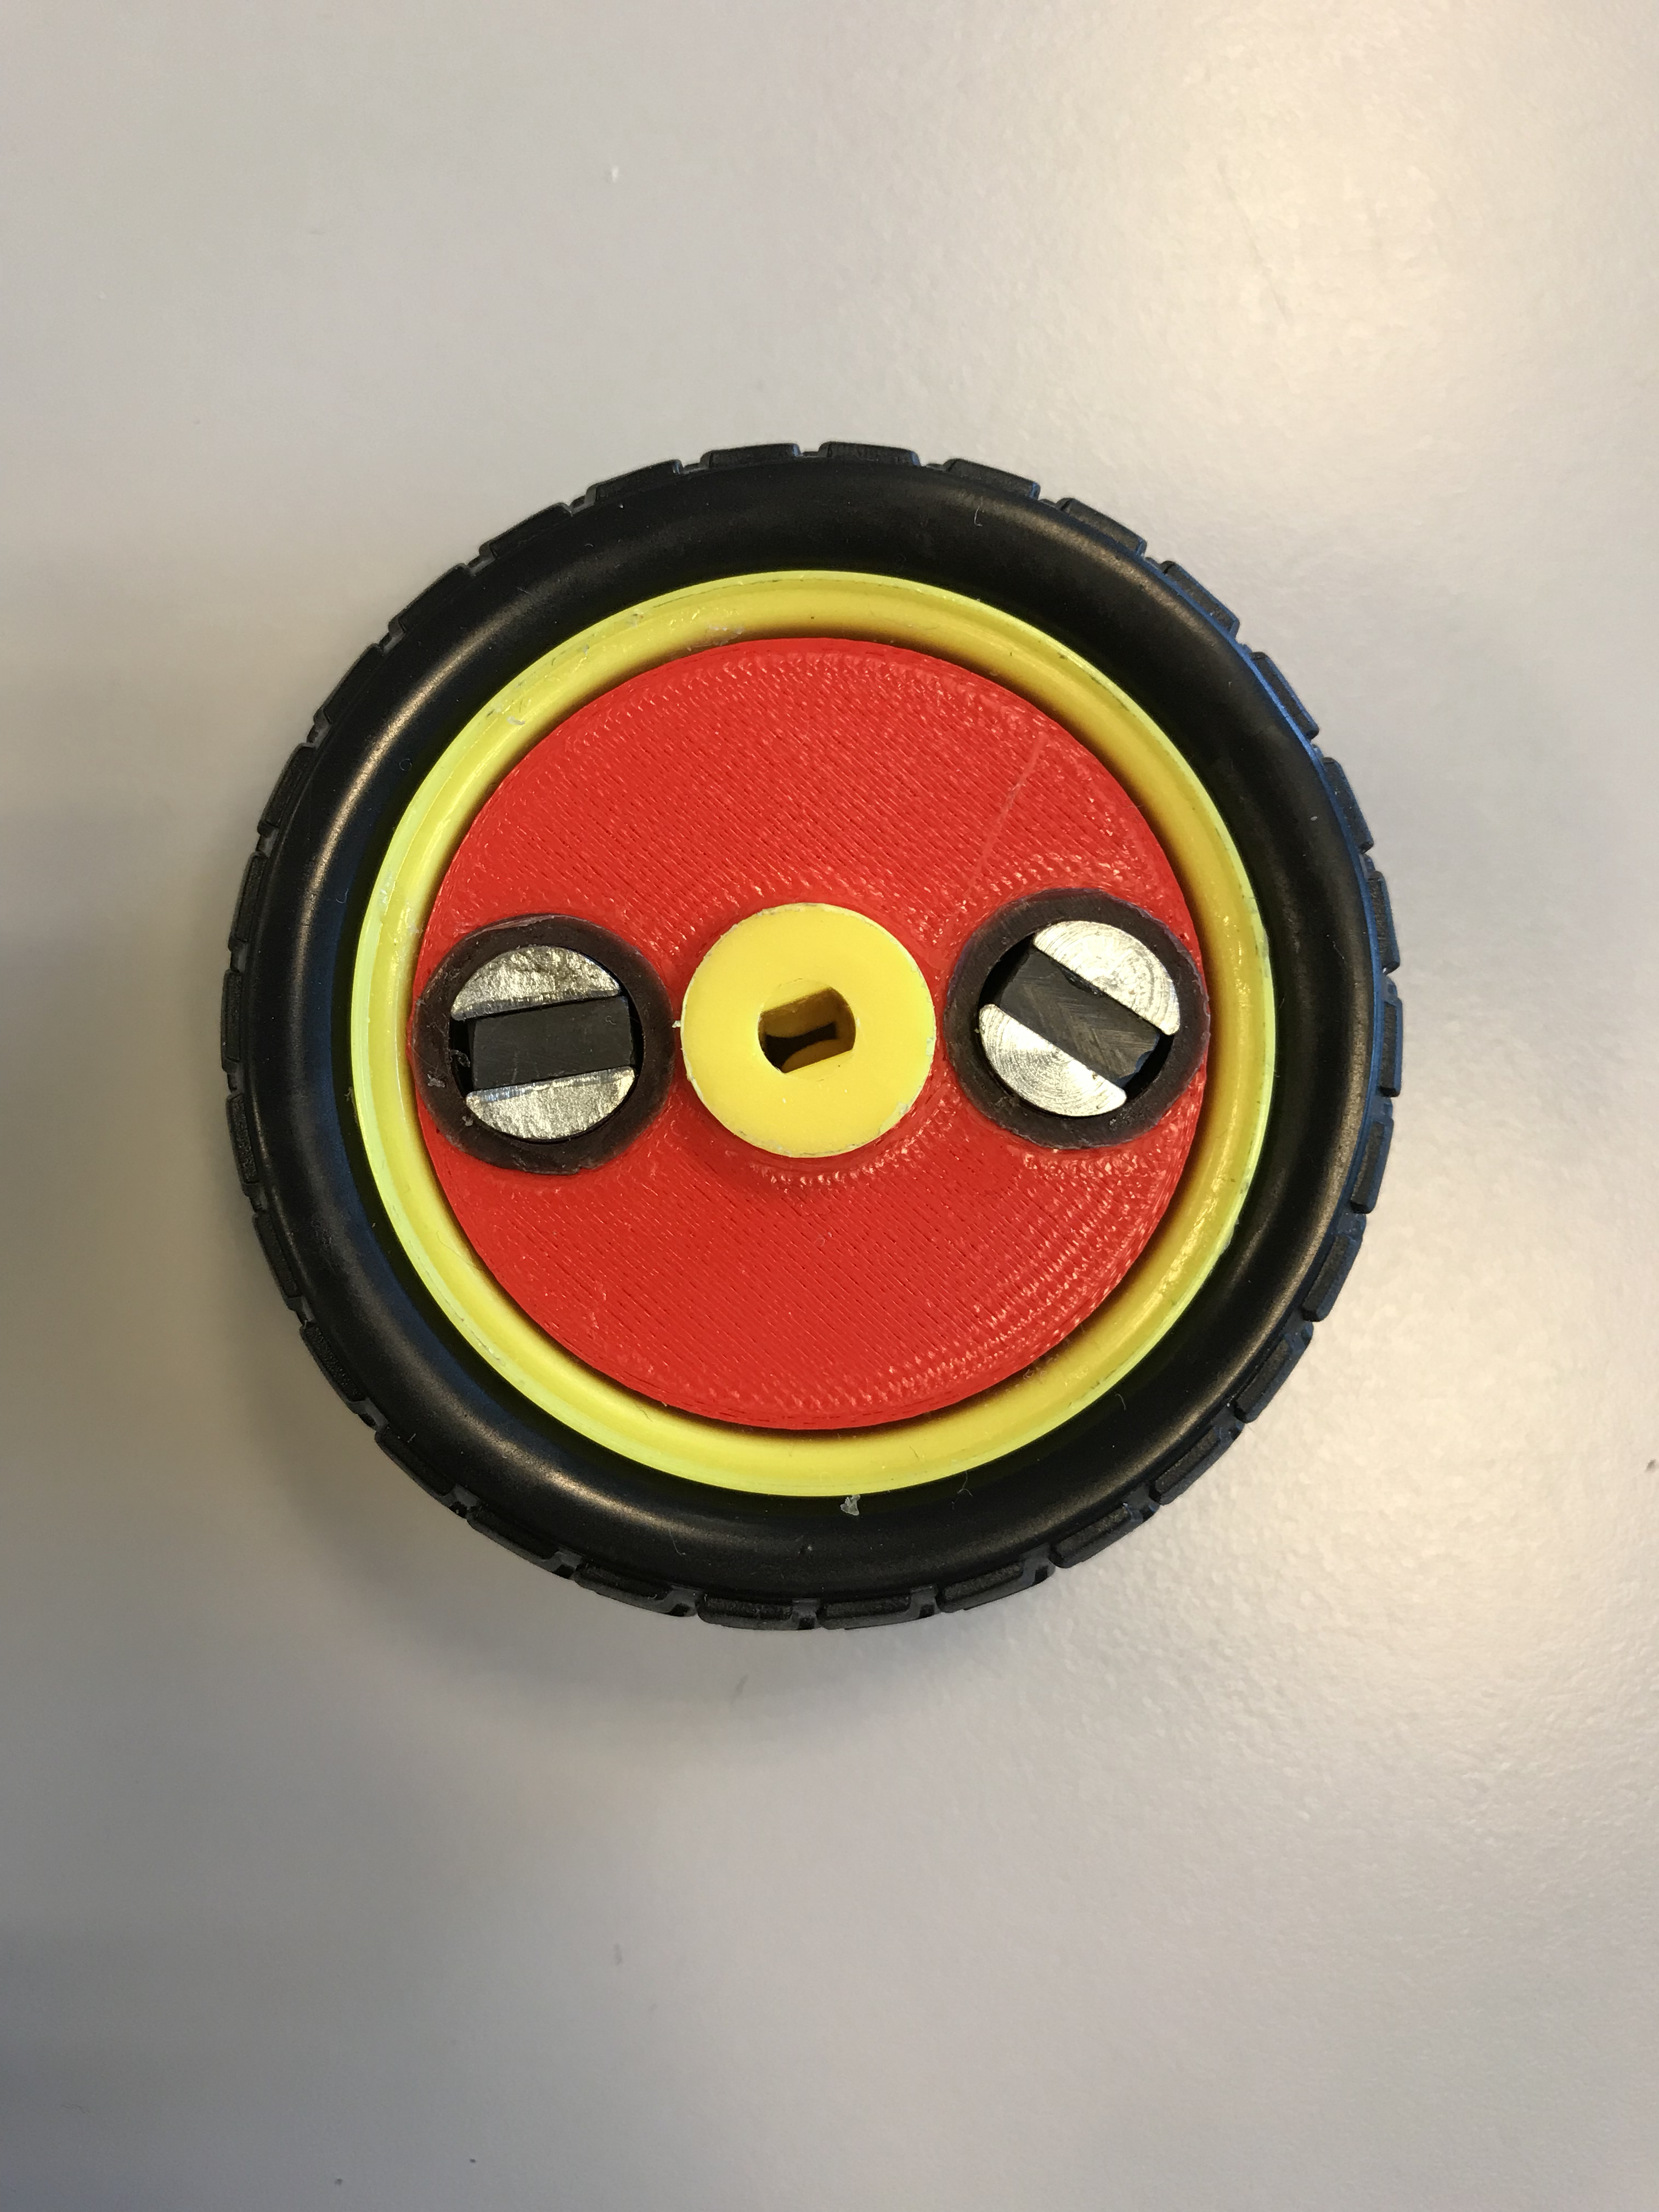
\includegraphics[width=0.7\textwidth,height=0.7\textheight,keepaspectratio]{wielmagneten.png}
	\end{column}
	\begin{column}{0.5\textwidth}  
		\begin{center}
			\includegraphics[width=\textwidth,height=0.7\textheight,keepaspectratio]{hallsensor.png}
		\end{center}
	\end{column}
\end{columns} 
\end{frame}

%%%%%%%%%%%%%%%%%%%%%%%%%%%%%%%%%%%%%%%%%%%%%%%%%%%%%%%%%%%%%%%%%%%%%%%%%%%%%%%%%%
\section{RFID reader}
\begin{frame}{RFID reader: PN532 van Elechouse}
\begin{columns}
	\begin{column}{0.5\textwidth}
		\begin{itemize}
			\item[] I\textsuperscript{2}C, SPI en HSU interfaces voorzien
			\item[] Libraries van Elechouse
			\item[] We gebruiken I\textsuperscript{2}C
		\end{itemize}
	\end{column}
	\begin{column}{0.5\textwidth}  
		\begin{center}
			\includegraphics[width=\textwidth,height=0.7\textheight,keepaspectratio]{rfidlezermontage.png}
		\end{center}
	\end{column}
\end{columns} 
\end{frame}

%%%%%%%%%%%%%%%%%%%%%%%%%%%%%%%%%%%%%%%%%%%%%%%%%%%%%%%%%%%%%%%%%%%%%%%%%%%%%%%%%%
\section{Bluetooth communicatie}
\begin{frame}{Bluetooth-communicatie met HC05}
\begin{columns}
	\begin{column}{0.5\textwidth}
		\begin{itemize}
			\item[] Arduino als slave
			\item[] Raspberry Pi als master
		\end{itemize}
	\end{column}
	\begin{column}{0.5\textwidth}  
		\begin{center}
			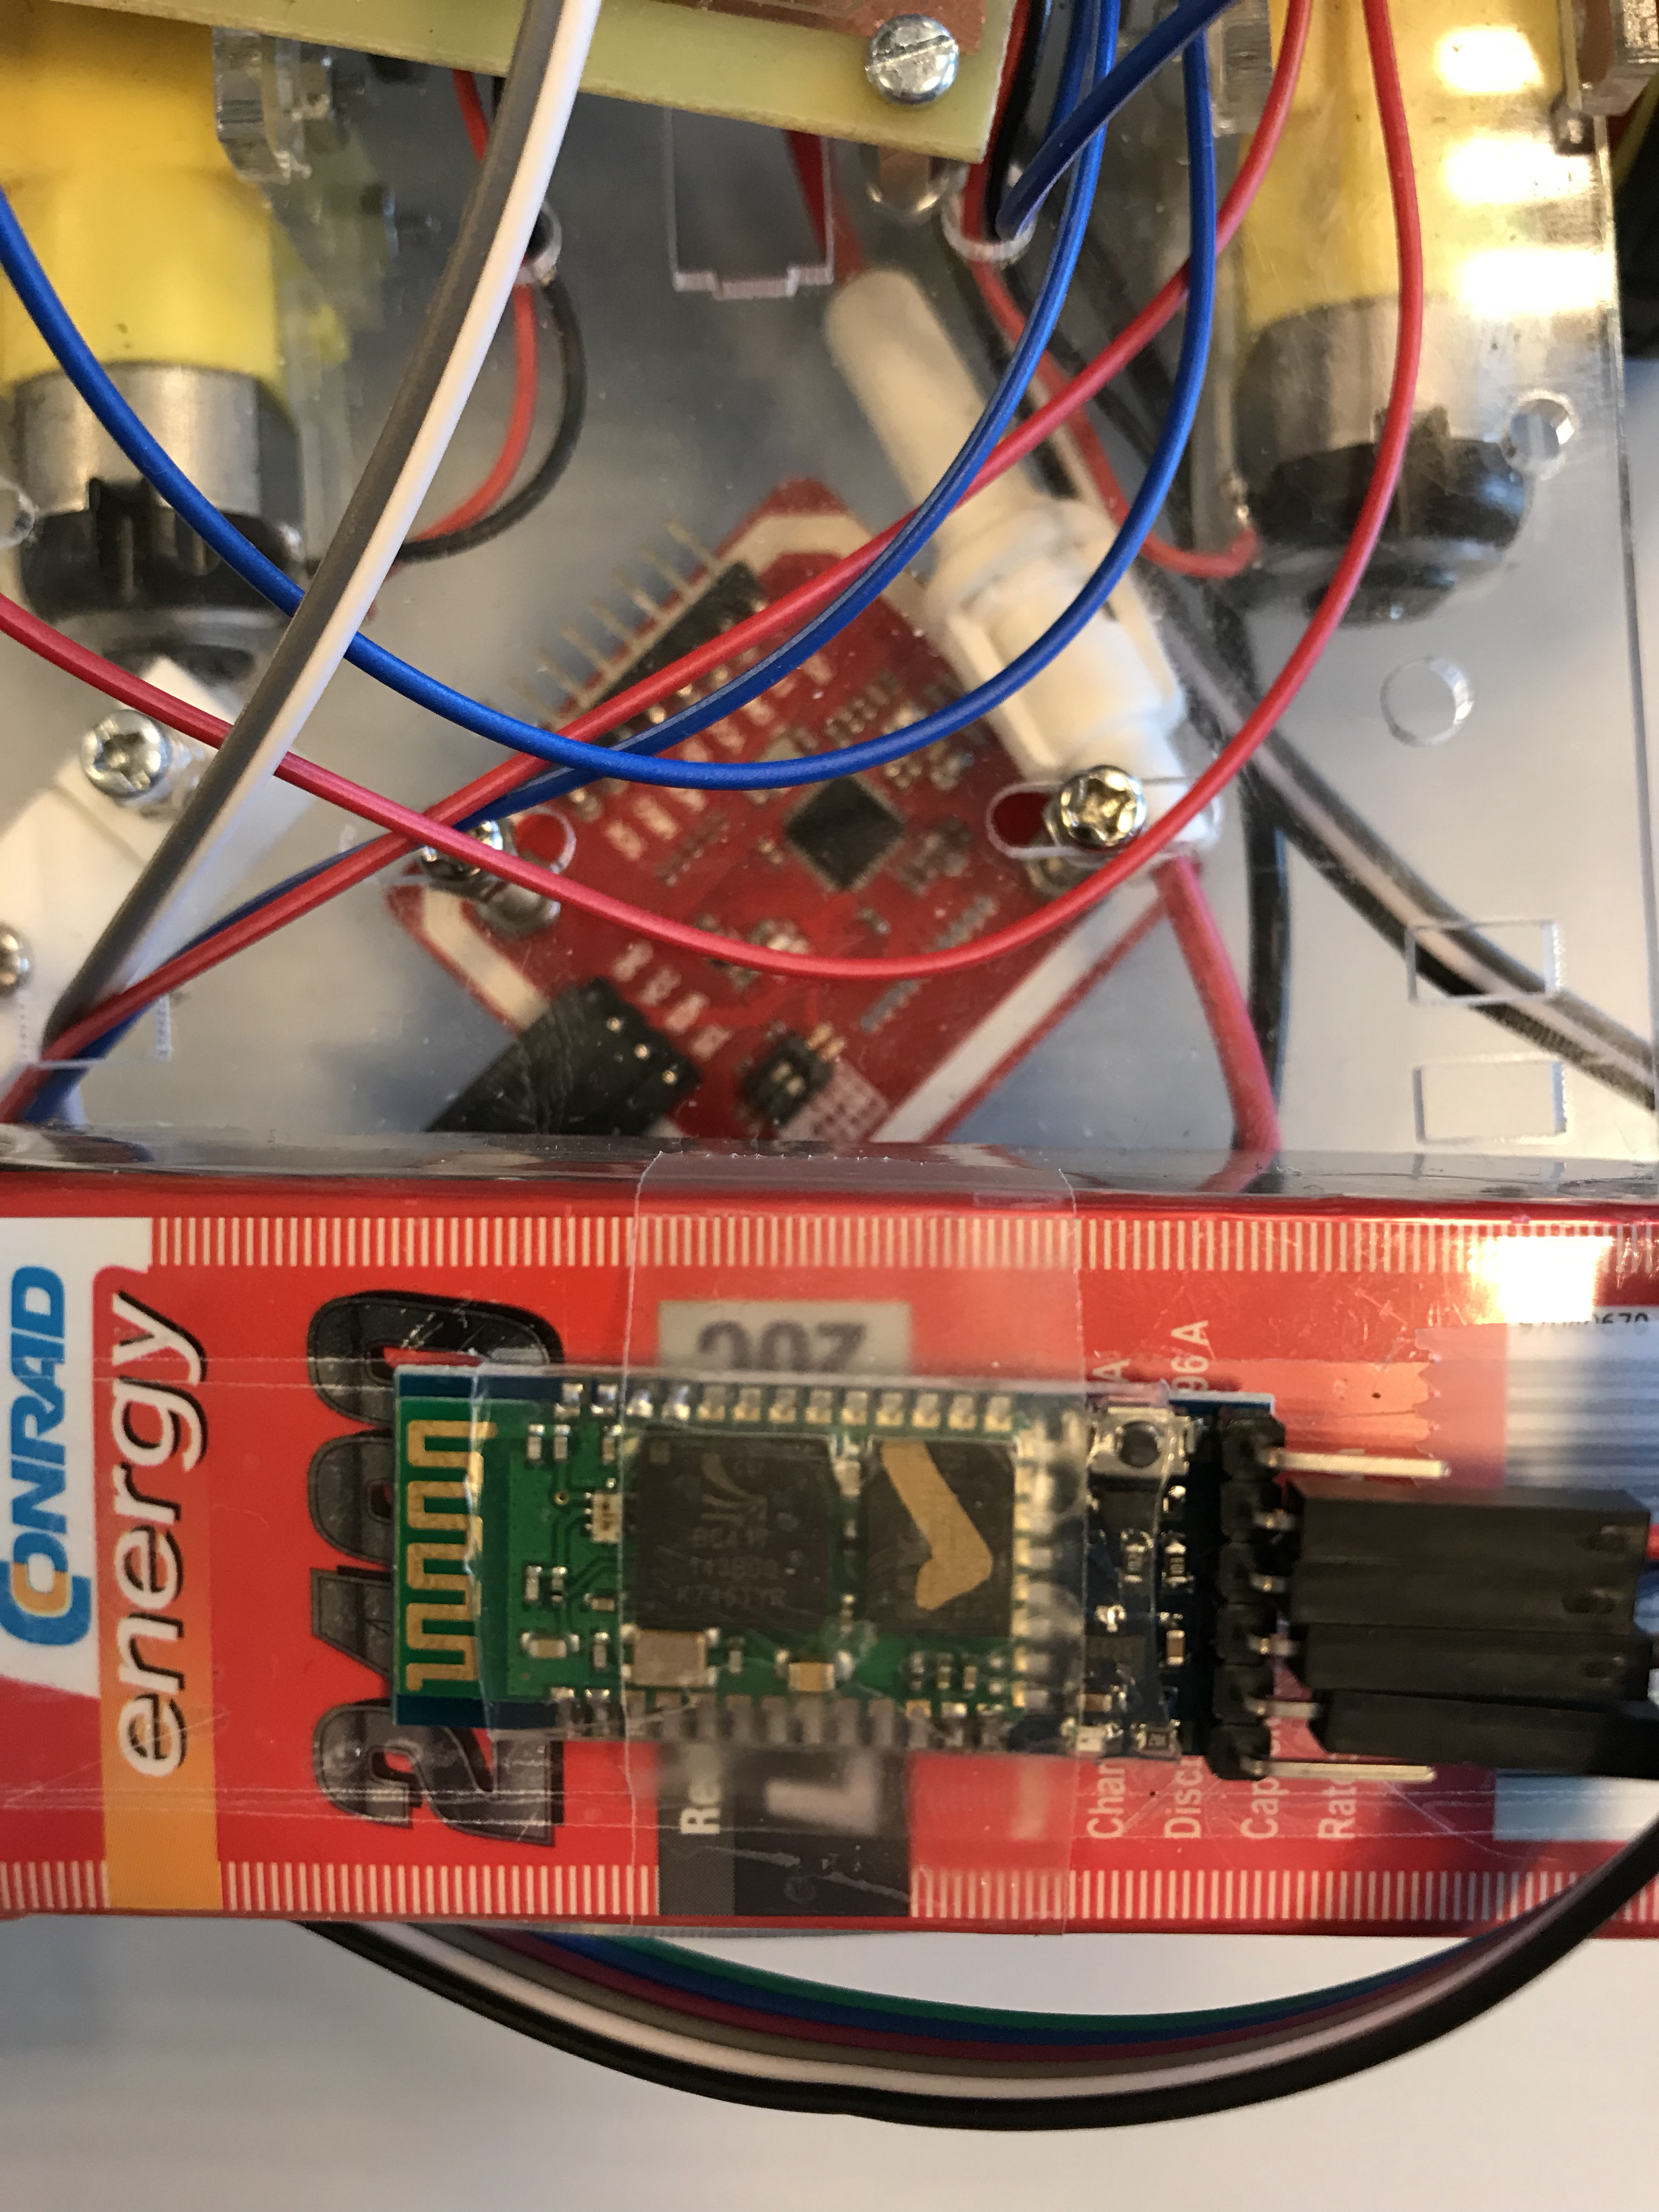
\includegraphics[width=\textwidth,height=0.7\textheight,keepaspectratio]{bluetoothenrfidlezer.png}
		\end{center}
	\end{column}
\end{columns} 
\end{frame}

\begin{frame}{}
\begin{figure}[H]
	\centering
	\includegraphics[width=\textwidth,height=0.8\textheight,keepaspectratio]{bluetoothoutputvoorbeeldbijgesneden2.png}
\end{figure}
\end{frame}

%%%%%%%%%%%%%%%%%%%%%%%%%%%%%%%%%%%%%%%%%%%%%%%%%%%%%%%%%%%%%%%%%%%%%%%%%%%%%%%%%%
\section{Software flowchart}
\begin{frame}{Software flowchart}
\begin{figure}[H]
	\centering
	\includegraphics[width=\textwidth,height=0.8\textheight,keepaspectratio]{arduinoflowchartpresentatie.png}
\end{figure}
\end{frame}


%%%%%%%%%%%%%%%%%%%%%%%%%%%%%%%%%%%%%%%%%%%%%%%%%%%%%%%%%%%%%%%%%%%%%%%%%%%%%%%%%%
\section{Besluit}
\title{}
\setbeamertemplate{background canvas}[title]

\begin{frame}[plain,noframenumbering]
\titlepage
\end{frame}

\usedefaultcanvas

\end{document}
